\documentclass[12pt]{article}
\usepackage{amssymb,amsmath}
\usepackage{graphicx}
\newcommand{\eq}[1]{\begin{align*}#1\end{align*}}
\newcommand{\on}[1]{\operatorname{#1}}
\title{Homework 2}
\author{Jeff Wendling}
\date{October 18, 2011}
\begin{document}
\maketitle
\section*{Problem 1}
We consider
\eq{
	I(x) &= \int_0^1 \sin(x[t + \frac{1}{6}t^3 - \sinh(t)])\cos t dt\\
	&= \on{Im}\int_0^1 \cos t e^{ix(t + \frac{1}{6}t^3 - \sinh(t))} dt
}
And so $\psi(t) = t + \frac{1}{6}t^3 - \sinh(t)$. Noticing the Taylor expansion of $\sinh$ we can see that
\eq{
	\psi^{(n)}(0) &= 0 \;\;\;\forall n < 5\\
	\psi^{(5)}(0) &= -1
}
Thus
\eq{
	I(x) &\approx \on{Im}\int_0^\infty 1\cdot e^{ix(0 + -\frac{t^5}{5!})} dt\\
	&\approx \on{Im}\int_0^\infty e^{-ix\frac{t^5}{5!}}\\
	&\approx \on{Im} e^{-i\frac{\pi}{10}} \left[\frac{5!}{x}\right]^{\frac{1}{5}} \frac{\Gamma(\frac{1}{5})}{5}\\
	&\approx -\sin(\frac{\pi}{10})\frac{\Gamma(\frac{1}{5})}{5}(5!)^\frac{1}{5}x^{-\frac{1}{5}}
}
\section*{Problem 2}
We consider the Airy integral,
\eq{
	Ai(\lambda) &= \frac{1}{2\pi i}\int_C e^{\lambda z - \frac{1}{3}z^3}dz
}
and make the change of variables, $\lambda = a^2$, and $z = at$ with $a > 0$ giving
\eq{
	\frac{1}{2\pi i}\int_C e^{\lambda z - \frac{1}{3}z^3}dz &= \frac{1}{2\pi i}\int_C e^{a^3t - a^3t^3/3}dt\\
	&= \frac{a}{2\pi i}\int_C e^{a^3(t - t^3/3)}dt
}
If we let $a^3 = x$ we have
\eq{
	\frac{a}{2\pi i}\int_C e^{a^3(t - t^3/3)}dt &= \frac{x^{1/3}}{2\pi i}\int_C e^{x(t - t^3/3)} dt
}
Now $p(t) = t - \frac{t^3}{3}$, and if $t = u + iv$ then
\eq{
	p(t) &= \phi(t) + i\psi(t)\\
	p(t) &= [u(1+v^2) - \frac{u^3}{3}] + i[v(1-u^2) + \frac{v^3}{3}]
}
Seeking a saddle point we find $t = 1 + i0$ and $t = -1 + i0$.
Considering the point $t = -1$ we see that $\psi(-1) = 0$ and so the constant phase contour satisfies
\eq{
	0 &= v(1-u^2) + \frac{v^3}{3}
}
So $v = 0$ or $v^2 = 3u^2 - 3$. Substituting both into $\phi$ we can see that the second curve has the steepest descent.
Rather than integrate along this curve we will approximate it by the curve
\eq{
	t &= -1 + is
}
Doing this substitution we see
\eq{
	\frac{x^{1/3}}{2\pi i}\int_C e^{x(t - t^3/3)} dt &\approx \frac{x^{1/3}}{2\pi} \int_{-\infty}^\infty e^{x(-\frac{2}{3} - s^2)} ds\\
	&\approx \frac{x^{1/3}}{2\pi}e^{-\frac{2}{3}x}\int_{-\infty}^\infty e^{-xs^2}ds\\
	&\approx \frac{x^{1/3}}{2\pi}e^{-\frac{2}{3}x}\sqrt{\frac{\pi}{x}}\\
	&\approx \frac{e^{-\frac{2}{3}x}}{2\sqrt{\pi}x^{1/6}}
}
Which turning back into $\lambda$ yields
\eq{
	Ai(\lambda) \approx \frac{e^{-\frac{2}{3}\lambda^{3/2}}}{2\sqrt{\pi}\lambda^{1/4}}
}
\section*{Problem 3}
\subsection*{Part (a) (stationary phase)} By directly applying (6.5.12) from the book with $p = 2$, we see
\eq{
	I(x) = \int_0^1 e^{ixt^2} dt &\approx e^{i\frac{\pi}{4}} \left[\frac{2!}{x|2|}\right]^\frac{1}{2} \frac{\Gamma(\frac{1}{2})}{2}\\
	&\approx e^{i\frac{\pi}{4}} \frac{1}{2\sqrt{x}} \sqrt{\pi}\\
	&\approx e^{i\frac{\pi}{4}} \sqrt{\frac{\pi}{4x}}
}
\subsection*{Part (b) (steepest descent)} Seeing that
\eq{
	p(t) &= it^2\\
	&= i(u + iv)^2\\
	&= i(u^2 + 2iuv - v^2)\\
	&= -2uv + i(u^2 - v^2)
}
Finding a constant phase contour through the point $t = 0$ we see that
\eq{
	\on{Im} p(0) = 0
}
So the constant phase contours satisify $u^2 = v^2$ so $u = v$ or $u = -v$. We can see that when $u = v$
\eq{
	\on{Re} p(t) = -2v^2
}
and so is the steepest descent. Performing the same analysis at $t = 1$ we find the steepest descent contour satisfies
\eq{
	u = \sqrt{v^2 + 1}
}
The original contour cannot be continuously deformed into these two contours because they have different imaginary parts, thus we must join them with
a straight line between them. The integral over this must be zero as the countours go to infinity because the length of the line connecting them will
approach zero. Thus we just need to consider the two contours given above.
\eq{
	I(x) &= \int_0^1 e^{ixt^2} dt\\
	&= \int_{C_1} e^{ixt^2} dt + \int_{C_2} e^{ixt^2}\\
}
Considering the first contour we have $t = (1+i)v$ and so
\eq{
	\int_{C_1} e^{ixt^2} &= (1+i)\int_0^\infty e^{-2xv^2} dv\\
	&= \frac{1+i}{\sqrt{2}} \int_0^\infty e^{-xv^2} dv\\
	&= \frac{1+i}{\sqrt{2}} \frac{1}{2}\sqrt{\frac{\pi}{x}}\\
	&= \frac{1}{2}\sqrt{\frac{\pi}{x}}e^{i\frac{\pi}{4}}
}
Considering the second contour we have $t = \sqrt{v^2 + 1} + iv$ and so
\eq{
	p(t) = i - 2v\sqrt{v^2 + 1}
}
So we change variables $p(t) = i - s$ where $s = 2v\sqrt{v^2 + 1}$, yielding
\eq{
	\int_{C_3} e^{ixt^2} dt &= \frac{1}{2}ie^{ix} \int_0^\infty (1 + is)^{-\frac{1}{2}} e^{-xs} ds
}
and apply Watson's Lemma with the Taylor expansion
\eq{
	(1 + is)^{-\frac{1}{2}} = \sum_{n=0}^\infty \frac{(-is)^n\Gamma(n + \frac{1}{2})}{n!\Gamma(\frac{1}{2})}
}
So
\eq{
	a_n &= \frac{(-i)^n\Gamma(n + \frac{1}{2})}{n!\Gamma(\frac{1}{2})}\\
	\beta_n &= n + \frac{1}{2}\\
	\alpha &= -\frac{1}{2}
}
Thus by Watson's Lemma,
\eq{
	I_3(x) &\approx \frac{1}{2}ie^{ix}\sum_{n=0}^\infty \frac{a_n\Gamma(\alpha + \beta_n + 1)}{x^{\alpha + \beta_n + 1}}\\
	&\approx \frac{1}{2}ie^{ix}\sum_{n=0}^\infty \frac{(-i)^n \Gamma(n + \frac{1}{2}) \Gamma(n + 1)}{n!\Gamma(\frac{1}{2}) x^{n+1}}\\
	&\approx \frac{1}{2\sqrt{\pi}}ie^{ix}\sum_{n=0}^\infty \frac{(-i)^n \Gamma(n + \frac{1}{2})}{x^{n+1}}
}
And so the full expansion is
\eq{
	I(x) \approx \frac{1}{2}\sqrt{\frac{\pi}{x}}e^{i\frac{\pi}{4}} - \frac{i}{2x}e^{ix} + ...
}
\section*{Problem 4}
\subsection*{Expansion of $\epsilon y'' + yy' - y = 0$} For the outer solution, we solve
\eq{
	yy' - y &= 0\\
	y' &= 1\\
	y &= x + 1
}
After applying the boundary condition $y(1) = 2$.
For the inner solution we let
\eq{
	\bar{x} = \frac{x}{\epsilon^\alpha}
}
so
\eq{
	\epsilon^{1-2\alpha}Y'' + Y\epsilon^{-\alpha} Y' - Y = 0
}
Which requires $1-2\alpha = -\alpha \implies \alpha = 1$. Thus we solve
\eq{
	Y'' + YY' &= 0\\
	Y'' + (\frac{Y^2}{2}) &= 0\\
	2Y' + Y^2 &= C_1^2\\
	2\frac{dY}{d\bar{x}} &= C_1^2 - Y^2\\
	\frac{dY}{C_1^2 - Y^2} &= \frac{1}{2}d\bar{x}\\
	\frac{1}{C_1}\tanh^{-1}(\frac{Y}{C_1}) &= \frac{1}{2}\bar{x} + C_2\\
	Y &= C_1\tanh(\frac{1}{2}\bar{x} C_1)
}
after applying the boundary condition $Y(0) = 0$. To match we let
\eq{
	x_\eta &= \frac{x}{\epsilon^\beta}
}
and
\eq{
	y_{\on{outer}} &= \epsilon^\beta x_\eta + 1 \rightarrow 1\;\on{as}\;x\rightarrow 0\\
	y_{\on{inner}} &= c\tanh(\frac{1}{2}\epsilon^{\beta - 1}x_\eta c) \rightarrow c\;\on{as}\;\bar{x}\rightarrow \infty
}
Thus $c = 1$ and $y_{\on{match}} = 1$ which yields
\eq{
	y_{\on{unif}} &= x + \tanh(\frac{x}{2\epsilon})
}
\subsection*{Expansion of $\epsilon y'' - (2x+1)y' + 2y = 0$}
For the outer we solve
\eq{
	2y &= (2x+1)y'\\
	\frac{dy}{2y} &= \frac{dx}{2x+1}\\
	\ln y &= \ln (2x + 1) + c\\
	y &= c(2x + 1)\\
	y = 2x + 1
}
after applying $y(0) = 1$. For the inner solution we let
\eq{
	\bar{x} = \frac{1 - x}{\epsilon^\alpha}
}
and find
\eq{
	\epsilon^{1-2\alpha}Y'' - (2 - 2\epsilon^\alpha\bar{x} + 1)\epsilon^{-\alpha}Y' + 2y = 0
}
and so $\alpha = 1$ which yields the ODE
\eq{
	Y'' - 3Y' = 0
}
with characteristic equation $m(m-3) = 0$, so
\eq{
	Y &= c_1 e^{-3\bar{x}} + c_2\\
	&= c(e^{-3\bar{x}} - 1)
}
after applying $y(1) = 0$. To find the matched solution we notice
\eq{
	y_{\on{outer}} &= 3\;\on{as}\;x \rightarrow 1\\
	y_{\on{inner}} &= -c\;\on{as}\;\bar{x} \rightarrow \infty
}
Thus $c = -3$ and $y_{\on{match}} = 3$, so
\eq{
	y_{\on{unif}} = 2x + 1 - 3e^{-\frac{3}{\epsilon}(1-x)}
}
Graphs comparing these results are attached.
\begin{table}[l]
	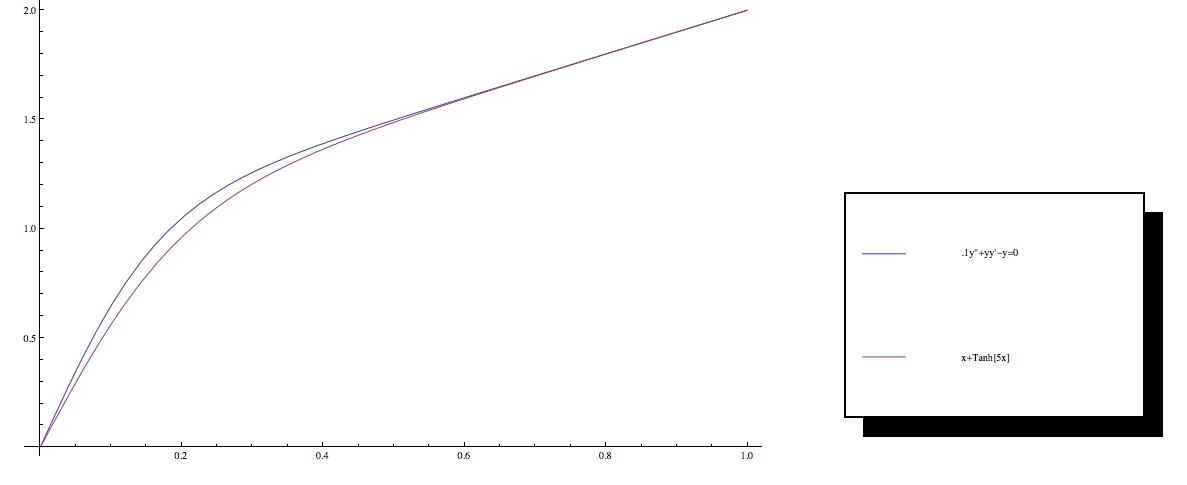
\includegraphics[width=6in]{graph1.jpg}\\
	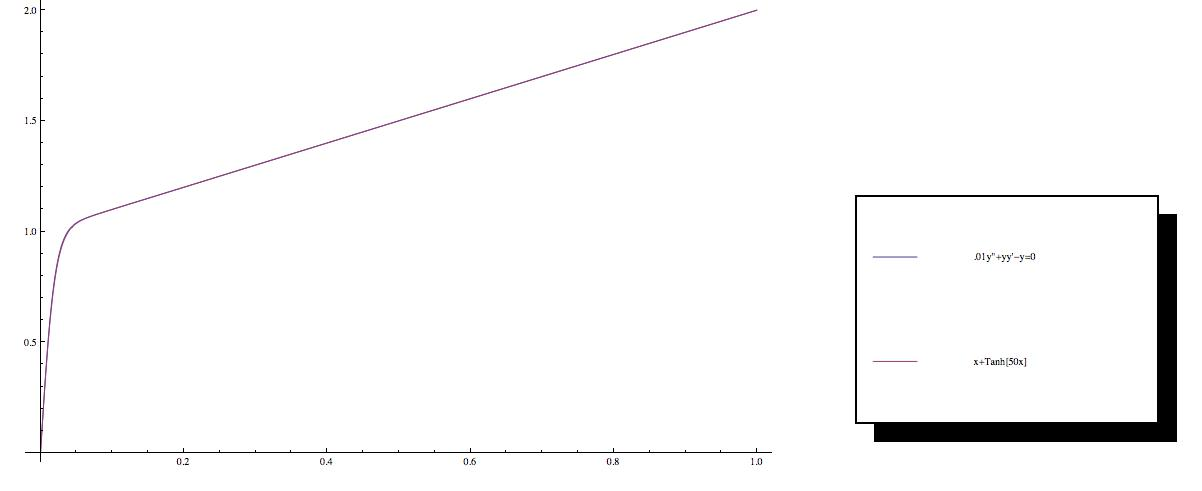
\includegraphics[width=6in]{graph2.jpg}
\end{table}
\newpage
\begin{table}[c]
	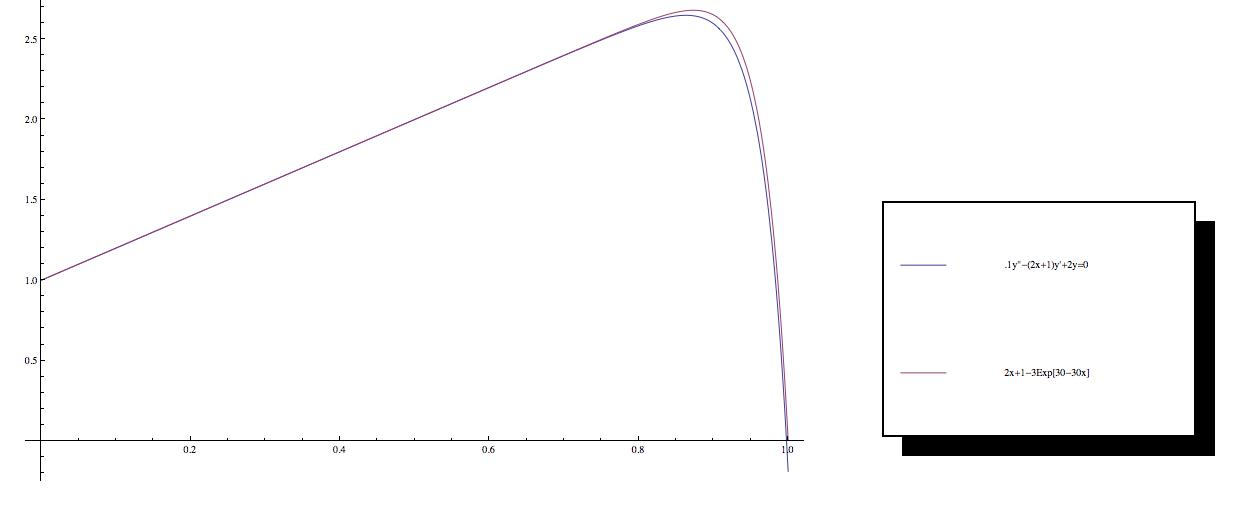
\includegraphics[width=6in]{graph3.jpg}\\
	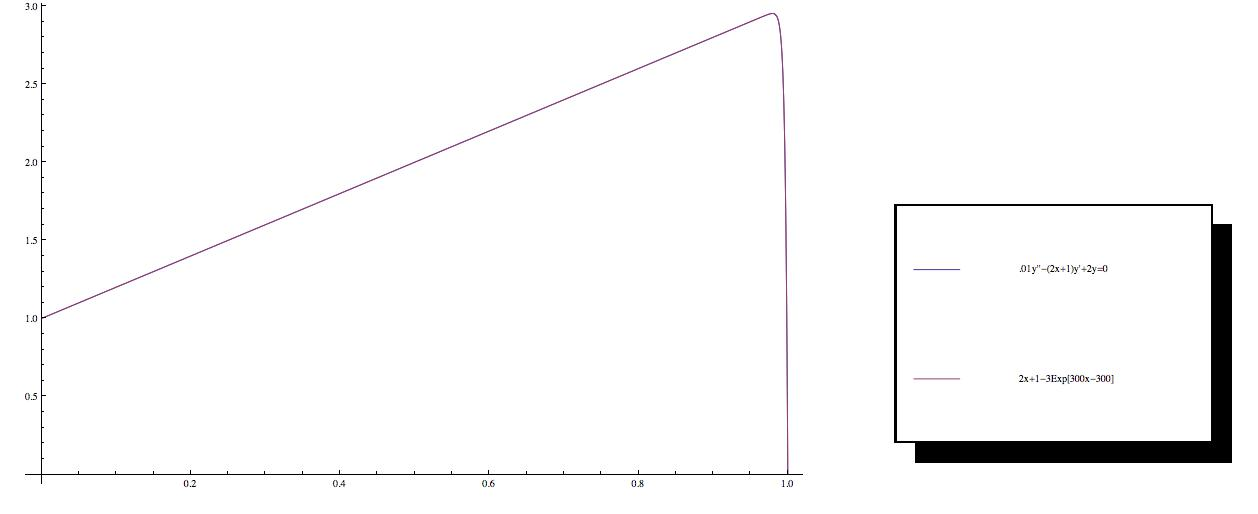
\includegraphics[width=6in]{graph4.jpg}
\end{table}
\end{document}